This Section describes the \gls{He} transport model and the grouped approach employed to simplify it.

\subsection{Helium clustering model}

This model describes the evolution of the concentrations of pure interstitial \gls{He} clusters (He$_x$) and mixed \gls{He}-vacancies clusters (He$_x$V$_y$) that are formed by \gls{trap mutation} events.
\begin{figure*}
    \centering
    \begin{overpic}[width=0.7\linewidth]{Figures/Chapter2/He clustering.pdf}
        \put(10, 60){He$_1$}
        \put(25, 60){He$_2$}
        \put(45, 60){He$_3$}
        \put(60, 60){He$_4$}
        \put(85, 60){V$_1$He$_7$}
        \put(78, 15){V$_1$He$_8$}
        \put(50, 15){V$_1$He$_9$}
        \put(22, 15){V$_2$He$_{10}$}
        
    \end{overpic}
    \caption{Representation of \gls{He} clustering in solids. Dissociation is omitted for simplification purposes. The thickness of the grey arrows represents the magnitude of the reaction rate between mobile He$_1$ and other clusters at the same distance.}
    \labfig{clustering sketch}
\end{figure*}


The spatio-temporal evolution of each species of size $i$ is defined by:
\begin{equation}
    \frac{\partial c_i}{\partial t} =  \nabla \cdot (D_i\nabla c_i) + \Gamma_i + R_i
    \labeq{model}
\end{equation}
In \refeq{model}, the first term of the right hand-side is the diffusion term where ${D=D_0 \cdot \exp\big(-E_\mathrm{diff}/ (k_B \cdot T )\big)}$ is the thermally activated diffusion coefficient expressed in \si{m^2.s^{-1}} with $E_\mathrm{diff}$ the diffusion activation energy in \si{eV}, $k_B$ the Boltzmann constant in \si{eV.K^{-1}} and $T$ the temperature in \si{K}.
If a species $i$ is assumed to be immobile, its diffusion coefficient $D_i$ is zero.
$\Gamma_i$ is the external production rate of species $i$.

The term $R_i$ is the coupling term due to reactions between species.
A simple reaction between two species can be described as:
\begin{equation}
    \ce{A + B <=>[k^+][k^-] AB}
\end{equation}

The forward rate constant $k^+_{A,B}$ is the clustering rate and is calculated using the theory of diffusion-limited reactions \sidecite{goldstein_diffusion_2007}:
\begin{equation}
    k^+_\mathrm{A,B} = 4 \pi (r_\mathrm{A} + r_\mathrm{B}) (D_\mathrm{A} + D_\mathrm{B})
\end{equation}
where $r_\mathrm{A}$ and $r_\mathrm{B}$ are the capture radii and $D_\mathrm{A}$ and $D_\mathrm{B}$ are the diffusion coefficients of species A and B respectively.
The backward rate constant $k^-_\mathrm{A,B}$ is the dissociation rate and is obtained using chemical equilibrium principles \cite{goldstein_diffusion_2007}:
\begin{equation}
    k^-_\mathrm{A,B} =\rho k^+_\mathrm{A,B}e^{\frac{-E_b}{k_B T}}
\end{equation}
where $\rho = \SI{6.3e28}{m^{-3}}$ is the atomic density of W in $\si{m^{-3}}$ and $E_b$ is the binding energy for the reaction \ce{AB -> A + B} in \si{eV}.

The reaction term $R_i$ is the coupling term between concentrations and is expressed as:

\begin{equation}
    R_i=  k^+_{i,i-1} c_1 c_{i-1}  - k_{i, 1}^+ c_i  c_{1} + k_{i+1}^- c_{i+1} -  k_i^- c_i
    \labeq{reaction term}
\end{equation}


In \refeq{reaction term}, $c_i$ is the concentration of clusters of size $i$ in \si{m^{-3}}.
The first term corresponds to the reactions producing clusters of size $i$.
The second one corresponds to the ones reacting with clusters of size $i$.
The third term accounts for bigger clusters dissociating.
Finally, the last term corresponds to clusters of size $i$ dissociating.

The system of equations can therefore be written as follows:

\begin{subequations}
    \begin{align}
        \frac{\partial c_1}{\partial t} &= \nabla \cdot (D_1 \nabla c_1) + \Gamma + \sum\limits_{i=2}^\infty k_{i}^- c_i - 2k_{1, 1}^+ c_1^2 - \sum\limits_{i=2}^\infty k_{1,i}^+ c_1 c_i \\
        \frac{\partial c_2}{\partial t} &= \nabla \cdot (D_2 \nabla c_2) - k_{1, 2}^+ c_1 c_2 + k_{1, 1}^+ c_1^2 - k_{2}^- c_2 + k_{3}^- c_3\\
        \vdots \nonumber\\
        \frac{\partial c_i}{\partial t} &= - k_{1, i}^+ c_1 c_i + k_{1, i-1}^+ c_1 c_{i-1} - k_{i}^- c_i\\
        \frac{\partial c_{i+1}}{\partial t} &= - k_{1, i+1}^+ c_1 c_{i+1} + k_{1, i}^+ c_1 c_i\\
        \vdots \nonumber
    \end{align}
    \labeq{temporal evolution no grouping}
\end{subequations}

\subsection{Grouped approach}
Extending this clustering model to clusters containing millions of helium extremely increases the computational cost.
A grouped approach proposed by Faney et al.\ \sidecite{faney_spatially_2014} for reducing the number of equations will therefore be employed.
This technique consists in grouping clusters from an arbitrary size $N$ in a single equation while explicitly accounting for smaller clusters.
To do so, the dissociation of large clusters is neglected (i.e.\ $k_i^- = 0$ for $i>N$).
This assumption is valid since the activation energy for \gls{trap mutation} events is lower than that of He or \gls{vacancy} emission\sidecite{boisse_modeling_2014}.
Dissociation of large clusters by \gls{vacancy} or He emission is therefore negligible.
Moreover, clusters containing more than six \gls{He} atoms are assumed to be immobile (i.e.\ $D_i = 0$ for $i>6$).
This assumption is motivated by \gls{dft} and \gls{md} results suggesting that the \gls{self-trapping} energy is below the binding energy of one He atom in a pure He cluster for clusters containing more than five He atoms \sidecite{boisse_modeling_2014}.

For smaller clusters ($\mathrm{He}_1$, $\mathrm{He}_2$,$\ldots$, $\mathrm{He}_6$) the diffusion coefficient and the dissociation by He emission energy vary with the number of \gls{He} atoms in the cluster (see \reftab{clusters properties}).

\refeq{temporal evolution no grouping} can therefore be written as:
\begin{subequations}
    \begin{align}
        \frac{\partial c_1}{\partial t} &= \nabla \cdot (D_1 \nabla c_1) + \Gamma + \sum\limits_{i=2}^N k_{i}^- c_i - 2k_{1, 1}^+ c_1^2 - \sum\limits_{i=2}^N k_{1,i}^+ c_1 c_i - \sum\limits_{i=N+1}^\infty k_{1,i}^+ c_1 c_i \\
        \frac{\partial c_2}{\partial t} &= \nabla \cdot (D_2 \nabla c_2) - k_{1, 2}^+ c_1 c_2 + k_{1, 1}^+ c_1^2 - k_{2}^- c_2 + k_{3}^- c_3\\
        \vdots \nonumber\\
        \sum\limits_{i=N}^\infty \frac{\partial c_{i}}{\partial t} &= k_{1, N}^+ c_1 c_N + \sum\limits_{i=N+1}^\infty k_{1, i}^+ c_1 c_i - \sum\limits_{i=N+1}^\infty k_{1, i}^+ c_1 c_i = k_{1, N}^+ c_1 c_N
    \end{align}
    \labeq{temporal evolution grouping no new symbols}
\end{subequations}

In order to simplify this set of equations, the following quantities are defined:

\begin{align}
    c_b &= \sum\limits_{i=N+1}^\infty c_i \quad \text{: bubbles concentration} \\
    \langle i_b \rangle &= \frac{1}{c_b} \sum\limits_{i=N+1}^\infty i c_i \quad \text{: average He content in bubbles} \\
    \langle r_b \rangle &=  \frac{1}{c_b}\sum\limits_{i=N+1}^\infty r_i c_i \quad \text{: average radius in bubbles}\\
    \langle k_b^+ \rangle &=  \frac{1}{c_b}\sum\limits_{i=N+1}^\infty k_{1,i}^+ c_i \quad \text{: average clustering rate in bubbles}
\end{align}
Clusters with more than $N$ \gls{He} ($c_b$) will be referred as ``bubbles'' in the following.

\refeq{temporal evolution grouping no new symbols} therefore reads:

\begin{subequations}
    \begin{align}
        \frac{\partial c_1}{\partial t} &= \nabla \cdot (D_1 \nabla c_1) + \Gamma + \sum\limits_{i=2}^N k_{i}^- c_i- 2k_{1, 1}^+ c_1^2 - \sum\limits_{i=2}^N k_{1,i}^+ c_1 c_i - \langle k_b^+ \rangle c_1 c_b \\
        \frac{\partial c_2}{\partial t} &= \nabla \cdot (D_2 \nabla c_2) - k_{1, 2}^+ c_1 c_2 + k_{1, 1}^+ c_1^2 - k_{2}^- c_2 + k_{3}^- c_3\\
        \vdots \nonumber\\
        \frac{\partial c_N}{\partial t} &= - k_{1, N}^+ c_1 c_N + k_{1, N-1}^+ c_1 c_{N-1} - k_{N}^- c_N\\
        \frac{\partial c_b}{\partial t} &= k_ {1,N}^+ c_1 c_N \\
    \end{align}
    \labeq{temporal evolution grouping}
\end{subequations}

The radius of pure \gls{He} clusters \sidecite{faney_spatially_2015} given by:
\begin{equation}
    r_{\mathrm{He}_x} = r_{\mathrm{He}_1} + \left(\frac{3}{4\pi} \frac{a_0^3}{10} x \right)^{1/3} - \left( \frac{3}{4\pi} \frac{a_0^3}{10} \right)^{1/3}
    \labeq{radius pure He}
\end{equation}
with $r_{\mathrm{He}_1} = \SI{0.3}{nm}$.

$\langle k_b^+ \rangle$ can be expressed as:
\begin{subequations}
    \begin{align}
        \langle k_b^+ \rangle &= \frac{1}{c_b}\sum\limits_{i=N+1}^\infty k_{1,i}^+ c_i\\
        &= \frac{1}{c_b} 4 \pi \sum\limits_{i=N+1}^\infty c_i  (r_1 + r_i) (D_1 + D_i)
    \end{align}
\end{subequations}

Assuming $D_i = 0$ for $i > N$:
\begin{subequations}
    \begin{align}
        \langle k_b^+ \rangle &= \frac{1}{c_b} 4 \pi D_1  \sum\limits_{i=N+1}^\infty c_i (r_1 + r_i) \\
        &= \frac{1}{c_b} 4 \pi D_1 \left(\sum\limits_{i=N+1}^\infty c_i r_1 + \sum\limits_{i=N+1}^\infty c_i r_i \right)\\
        &= \frac{1}{c_b} 4 \pi D_1 \left(r_1 c_b  + \sum\limits_{i=N+1}^\infty c_i r_i \right)\\
        &= 4 \pi D_1 (r_1 + \langle r_b \rangle) 
    \end{align}
\end{subequations}

For clusters containing both \gls{He} and vacancies, the radius only depends on the number of vacancies $m$ is given by \cite{faney_spatially_2015}:
\begin{equation}
    r_{\mathrm{He}_i\mathrm{V}_m} = r_{\mathrm{He}_0 \mathrm{V}_1} + \left(\frac{3}{4 \pi} \frac{a_0^3}{2} m \right)^{1/3} - \left(\frac{3}{4 \pi} \frac{a_0^3}{2} \right)^{1/3}
\end{equation}
with $a_0 = \SI{0.318}{nm}$ the lattice parameter and $r_{\mathrm{He}_0 \mathrm{V}_1} =  a_0 \sqrt{3}/4$.


The bubble radius $\langle r_b \rangle$ therefore reads:
\begin{subequations}
    \begin{align}
        \langle r_b \rangle &=  \frac{1}{c_b}\sum\limits_{i=N+1}^\infty  c_i \ r_{\mathrm{He}_i\mathrm{V}_m}\\
                            % &= r(\mathrm{He}_{\langle i_b \rangle}\mathrm{V}_{\langle i_b \rangle/4}) \\
        &= \frac{1}{c_b}\sum\limits_{i=N+1}^\infty c_i \left( r_{\mathrm{He}_0 \mathrm{V}_1} + \left(\frac{3}{4 \pi} \frac{a_0^3}{2} m \right)^{1/3} - \left(\frac{3}{4 \pi} \frac{a_0^3}{2} \right)^{1/3} \right)\\
        &= r_{\mathrm{He}_0 \mathrm{V}_1} + \left(\frac{3}{4 \pi} \frac{a_0^3}{2} \right)^{1/3} \frac{1}{c_b}\sum\limits_{i=N+1}^\infty c_i \ m^{1/3} - \left(\frac{3}{4 \pi} \frac{a_0^3}{2} \right)^{1/3}
    \end{align}
    \labeq{radius average}
\end{subequations}

The number of vacancies in bubbles $m$ is assumed to be $i/4$ (i.e.\ four helium per vacancy).
This assumption is motivated by \gls{md} computations showing that \gls{trap mutation} events occur for every four additional helium in large \gls{vacancy}-helium clusters.
Moreover, theoretical models for He bubbles growth in metals suggest a similar trend \sidecite{hammond_theoretical_2020}.

The average radius $\langle r_b \rangle$ therefore reads:
\begin{equation}
    \langle r_b \rangle = r_{\mathrm{He}_0 \mathrm{V}_1} + \left(\frac{3}{4 \pi} \frac{a_0^3}{2} \right)^{1/3} \frac{1}{c_b}\sum\limits_{i=N+1}^\infty c_i(\frac{i}{4})^{1/3} - \left(\frac{3}{4 \pi} \frac{a_0^3}{2} \right)^{1/3}
\end{equation}

Assuming $c_i$ follows a narrow gaussian distribution, $\frac{1}{c_b}\sum\limits_{i=N+1}^\infty c_i(\frac{i}{4})^{1/3} \approx \left( \frac{1}{c_b}\sum\limits_{i=N+1}^\infty c_i\frac{i}{4} \right)^{1/3} $ (see \reffig{sum of powers approximation}).
% is assumed to be only dependent on $\langle i_b \rangle$.

\begin{figure}
    \begin{subfigure}{0.75\linewidth}
        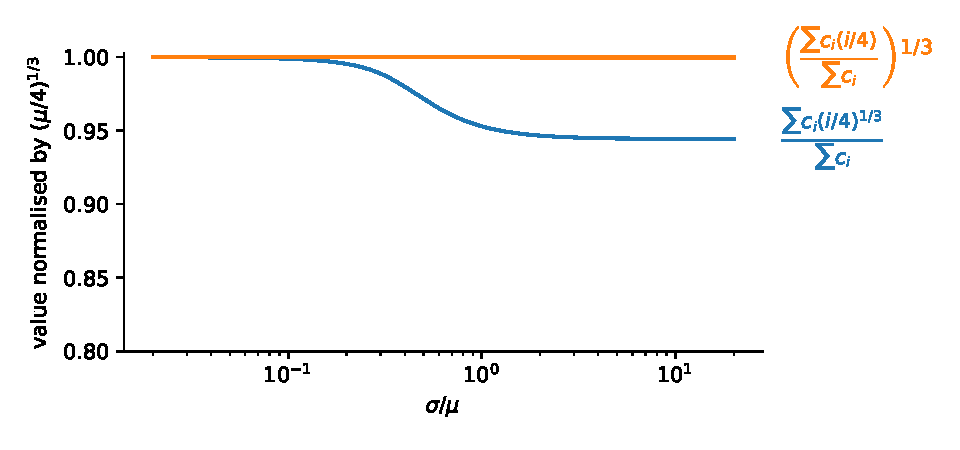
\includegraphics[width=\linewidth]{Figures/Chapter5/comparison_sum_of_powers_power_of_sums.pdf}
    \end{subfigure}%
    \begin{subfigure}{0.25\linewidth}
        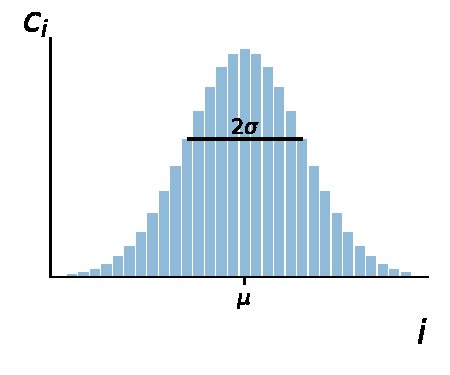
\includegraphics[width=\linewidth]{Figures/Chapter5/gaussian_representation.pdf}
    \end{subfigure}
    \caption{Validity of the sum approximation in the computation of the bubble radius assuming $c_i$ has a gaussian distribution centered on $\mu$ and with a standard deviation $\sigma$.}
    \labfig{sum of powers approximation}
\end{figure}


The final expression of the bubble radius is therefore:
\begin{equation}
    \langle r_b \rangle = r_{\mathrm{He}_0 \mathrm{V}_1} + \left(\frac{3}{4 \pi} \frac{a_0^3}{2} \frac{\langle i_b \rangle}{4} \right)^{1/3} - \left(\frac{3}{4 \pi} \frac{a_0^3}{2} \right)^{1/3}
\end{equation}

To solve for $\langle i_b \rangle$, is also useful to write the expression of the sum $\sum\limits_{i=N+1}^\infty i \frac{\partial c_i}{\partial t}$:

\begin{align}
    \sum\limits_{i=N+1}^\infty i \frac{\partial c_i}{\partial t} &= \sum\limits_{i=N+1}^\infty i k_{1,i-1}^+ c_1 c_{i-1} - \sum\limits_{i=N+1}^\infty i k_{1,i}^+ c_1 c_{i} \nonumber\\
    &= (N+1) k_{1,N}^+ c_1 c_N + \sum\limits_{i=N+2}^\infty i k_{1,i-1}^+ c_1 c_{i-1} - \sum\limits_{i=N+1}^\infty i k_{1,i}^+ c_1 c_{i} \nonumber\\
    &= (N+1) k_{1,N}^+ c_1 c_N + \sum\limits_{i=N+1}^\infty (i + 1) k_{1,i}^+ c_1 c_{i} - \sum\limits_{i=N+1}^\infty i k_{1,i}^+ c_1 c_{i} \nonumber\\
    &= (N+1) k_{1,N}^+ c_1 c_N + \sum\limits_{i=N+1}^\infty (i + 1) k_{1,i}^+ c_1 c_{i} - i k_{1,i}^+ c_1 c_{i} \nonumber\\
    &= (N+1) k_{1,N}^+ c_1 c_N + \sum\limits_{i=N+1}^\infty k_{1,i}^+ c_1 c_{i} \nonumber\\
    \frac{\partial \langle i_b \rangle c_b}{\partial t} &= (N+1) k_{1,N}^+ c_1 c_N + \langle k_b^+ \rangle c_1 c_b
    \labeq{pde for d (cb ib)/ dt}
\end{align}

The final form of the system of governing equations is obtained by adding \refeq{pde for d (cb ib)/ dt} to \refeq{temporal evolution grouping}:
\begin{subequations}
    \begin{align}
        \frac{\partial c_1}{\partial t} &= \nabla \cdot (D_1 \nabla c_1) + \Gamma + \sum\limits_{i=2}^N k_{i}^- c_i- 2k_{1, 1}^+ c_1^2 - \sum\limits_{i=2}^N k_{1,i}^+ c_1 c_i - \langle k_b^+ \rangle c_1 c_b \\
        \frac{\partial c_2}{\partial t} &= \nabla \cdot (D_2 \nabla c_2) - k_{1, 2}^+ c_1 c_2 + k_{1, 1}^+ c_1^2 - k_{2}^- c_2 + k_{3}^- c_3\\
        \vdots \nonumber\\
        \frac{\partial c_N}{\partial t} &= - k_{1, N}^+ c_1 c_N + k_{1, N-1}^+ c_1 c_{N-1} - k_{N}^- c_N\\
        \frac{\partial c_b}{\partial t} &= k_ {1,N}^+ c_1 c_N \\
        \frac{\partial (\langle i_b \rangle c_b)}{\partial t} &= (N+1)k_ {1,N}^+ c_1 c_N  + \langle k_b^+ \rangle c_1 c_b
    \end{align}
    \labeq{final system of equation}
\end{subequations}

The current implementation further simplifies Faney's model \sidecite{faney_spatially_2014}:
\begin{itemize}
    \item Interactions with \gls{self-interstitial} atoms or pre-existing vacancies are not taken into account.
    In this work, the only dissociations are He emissions from small mobile clusters and \gls{trap mutation} for large clusters.
    It was showed that this assumption did not have an impact on the results (see \reffig{tendril profiles}).
    \item The only clusters explicitly computed are $\mathrm{He}_{x \leq 6}$ (i.e.\ $N=6$) whereas Faney's work explicitly accounted for clusters up to $\mathrm{V}_{50}\mathrm{He}_{250}$ and solved a bigger system of equations.
    The influence of this threshold $N$ above which clusters are integrated in the quantity $c_b$ is discussed in \refsec{impact of N}.
\end{itemize}

\begin{table}
    \centering
    \begin{tabular}{L{1cm} R{2cm} R{1.6cm} R{1.1cm} R{1.6cm} R{1.1cm} R{2cm}}
        Cluster & $D_0 (\si{m^2 s^{-1}})$  & $E_\mathrm{diff} (\si{eV})$ &  $E_b (\si{eV})$   \\
        \hline
        \\
        He$_1$ & $2.95\times 10^{-8}$ & $0.13$ & - \\
        He$_2$ & $3.24\times 10^{-8}$ & $0.20$ & 1.0\\
        He$_3$ & $2.26\times 10^{-8}$ & $0.25$ & 1.5\\
        He$_4$ & $1.68\times 10^{-8}$ & $0.20$ & 1.5\\
        He$_5$ & $5.20\times 10^{-9}$ & $0.12$ & 1.6\\
        He$_6$ & $1.20\times 10^{-9}$ & $0.30$ & 2.0\\
    \end{tabular}
    \caption{Pure \gls{He} clusters properties in \gls{W}. Diffusion properties are taken from Faney et al.\ \cite{faney_spatially_2015} and binding energies are taken from Becquart et al.\ \cite{becquart_microstructural_2010}.}
    \labtab{clusters properties}
\end{table}

% for some reason, uncommenting this activates the top table
% \begin{table}
%  \begin{tabular}{ c c c c }
%  \toprule
%  col1 & col2 & col3 & col 4 \\
%  \midrule
%  \multirow{3}{4em}{Multiple row} & cell2 & cell3 & cell4\\ &
%  cell5 & cell6 & cell7 \\ &
%  cell8 & cell9 & cell10 \\
%  \multirow{3}{4em}{Multiple row} & cell2 & cell3 & cell4 \\ &
%  cell5 & cell6 & cell7 \\ &
% cell8 & cell9 & cell10 \\
%  \bottomrule
%  \end{tabular}
% \end{table}


This \gls{He} transport model was implemented in Python and solved using the finite element solving platform \gls{fenics} \sidecite{alnaes_fenics_2015}.
